\subsection{Systematic Date and Time Errors}\label{an:date} 
Correct time-stamps are critical in post election audits as they can preclude further log analysis. The data set used for this work was found to include many erroneous time-stamps. We found it simplest to classify these date errors into two categories: errors resulting from incorrectly set clocks and errors resulting from apparent bugs in the iVotronic time-stamp mechanism itself. Our website includes a report for each category and automatically identifies as many as these errors as possible while avoiding false positives.  

The iVotronic DREs append each audit event to the log in chronological order.  Each event is marked with a time-stamp based on the DRE's internal clock. Each DRE's clock is manually set by election officials or the iVotronic vendors. Any manual adjustments made to the clock are recorded on the audit log. Time-stamps should only change to reflect the passing of time unless the clock is manually set. The reports generated to detect and classify date errors are specific to the iVotronic audit logs in that they were tailored around some of the most common errors seen from this vendor.  The process could be applied to other logs assuming they maintain similar properties and modified for accuracy based on the data.  

Emphasis was placed on the accurate identification of date errors rather then complete identification. False positives create excessive amounts of data which would undermine the usefulness of the analysis. Determining the accuracy of time-stamps during a post-election audit can have a lot of ambiguities. If a machine has its clocks set an hour back it is difficult to determine if it opened early or if its clock is incorrectly set. For these reasons, techniques were developed in such as way as to avoid as many false identification of errors as possible.

All data was collected by sequentially parsing each time-stamp while looking for specific events such as manual time changes or erroneous shifts between time-stamps. A machine's open state was tracked by looking at terminal opening and closing events. Only the last set of openings and closings were considered for each machine. This helped ensure we were looking at election day statistics. Early voting was found to be conducted at inconsistant dates among the counties and was ignored for accuracy and relative importance of events such as manual time changes.


\subsubsection{Incorrectly Set Dates}
This report identifies any machine determined to open for election day voting with an incorrect clock.  This means the opening event and possibly all vote events were recorded with incorrect time-stamps. This can prevent other analyses from properly detecting how long the polls stayed open, whether they opened on time, or if they experienced long lines. Additionally, It may be useful for an election official to identify counties or precincts where these errors were particularly common so that pre-election testing procedures can be improved. There are two tables to categorize the results for this report.

The first table identified machines that had their clocks adjusted during election day voting. This caught machines that were only off by a couple hours as well as machines opening on election day with completlely incorrect dates.  Machines whose clock is only incorrect by a couple hours are difficult to identify because opening and closing times are not a consistant point of reference. Because of this ambiguity, only machines who were manually adjusted during election day were marked. The algorithm looked for a manual time adjustment event for any machine that was in an open state during election day.  If the machine then closed successfully on election day, the delta of the time change is recorded. This time delta can be used to correctly adjust the recorded opening time of the machine.

Figure~/ref{fig:Georgetown} shows an example of a 1 hour time change for the Georgetown county.  This county had 125 out of 140 machines adjusted nearly exactly one hour back in time.  This is presumably because the wrong DST algorithm was in use as mentioned in previous audits.~/cite{Buell2011}
\begin{figure}[h!]
  \caption{Resetting an iVotronic clock by one hour in Georgetown County}
  \label{fig:Georgetown}
  \centering
    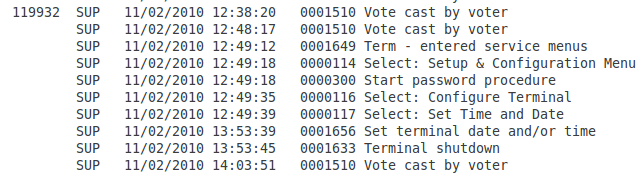
\includegraphics[width=0.5\textwidth]{datefig1.png}
\end{figure}

The second table found machines that opened on incorrect dates for voting but never had their clocks corrected.  In the first table clocks that were only slightly off were detected because someone changed the date during elections.  These small changes couldn't be detected if there wasn't an obvious manual adjustment. This table detected errors by looking for completely unprobable dates. This means dates a month or so before election day and any dates one or more days after election day.

\subsubsection{Datetime Errors}
The second report identifies anomalies in the time stamps that aren't a result of human error. We found many dates that changed seemingly at random and without a manual date adjustment event. These occurrences suggest an issue with the machine itself rather then procedural error. The cause of these errors remain unknown and have the potential to invalidate other audit statistics. It is concerning that these set values can change arbitrarily. Reporting these anomalies may assist offcials in determining which machines are experiancing errors to potentially report to the DRE vendor.

Many machines were found to exhibit odd behavior in which a clock would appear to temporarily or permantly shift its clock without human adjustment. This algorithm identifies these jumps.  In all the cases observed these jumps in clock values were significant enough to not be confused as the passing of time between two events in the log. 

Since events are appended in chronological order; any time-stamp that decreases chronologically without a manually date adjustment event is wrong and added to this category. Forward jumps in time are not necessarily the result of an inconsistent time record because a machine can be shut down for weeks between events.  Given the relatively short duration of elections, jumps forward in time that are past a certain threshold can reasonably be considered erroneous. The algorithm looked for deltas between time-stamps that jump forward by more then 33 days.  Using the 2010 South Carolina Data set, this seemed to avoid listing that are not obviously erroneous. Additionally, some machines were found to have their clock set to some type of null state where the clock stopped incrementing and marked blank dates. 

Once one of these odd changes in clock value is detected, the previous time-stamp is marked as the start and a counter increments on each subsequent event.  The counter ends and the anomaly is assumed to have ended based on criteria for each type of jump. The backward jump is presumed over if an event appears that is chronologically forward in time compared to the start event.  The forward jump is assumed over if an event appears on the same day of the starting event.  The zero clock anomaly is detected as returning to normal as soon as a non-zero date appears. The number of events associated with an anomaly is reported as well as the anomalous date and machine serial number. 

